\chapter{Tecnologías de manufactura aditiva}

\section{Introducción}

Llamaremos procesos de manufactura aditiva a todas las técnicas en las que el material se \textbf
{deposita/forma de manera controlada} y capa a capa sobre un volumen de trabajo para construir directamente geometrías tridimensionales. 

La construcción secuencial elimina restricciones de trayectoria (colisiones, cambios de herramienta) propias de máquinas-herramienta convencionales y fusiona varias etapas de fabricación en un único paso. Por ejemplo, en la Figura \ref{roki} se ilustran las ventajas en tiempo y costo al producir una cámara de empuje de cohete mediante manufactura aditiva frente a métodos convencionales. 

\begin{figure}[h!]
	\centering
	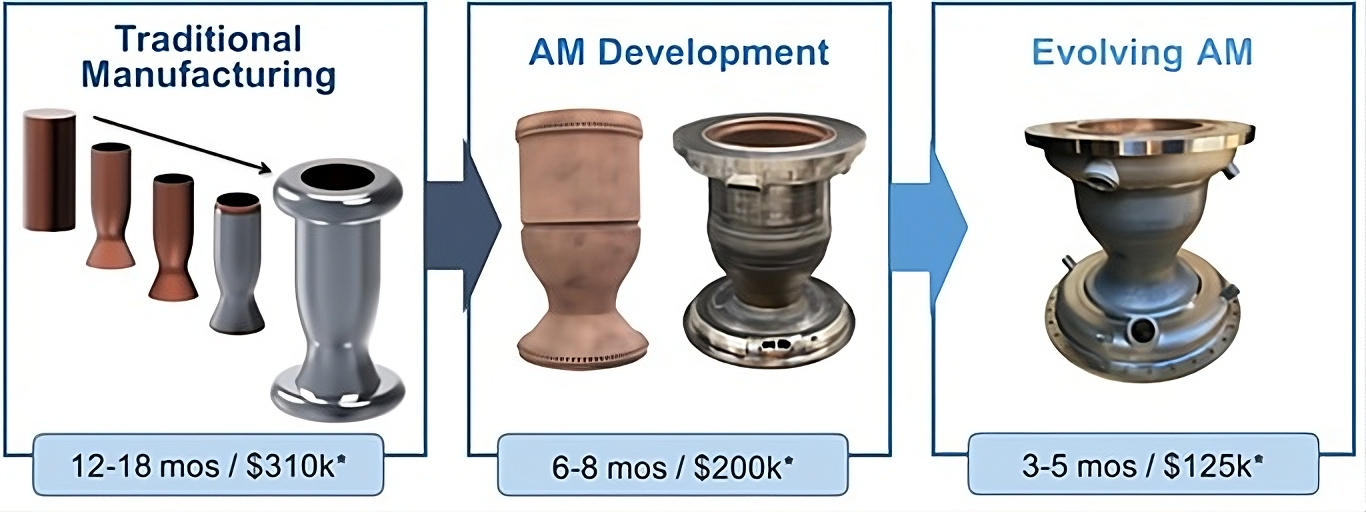
\includegraphics[width=0.8\linewidth]{imgs/rocket.png}
	\caption{Comparación de tiempos y costos de producción para la cámara de empuje de un cohete, de convencional a aditiva.\cite{rokeke}}
	\label{roki}
\end{figure}

Las tecnologías de manufactura aditiva suelen poseer las siguientes características en común:

\begin{description}

\item[Versatilidad geométrica]  
    No tienen restricciones de forma o un enfoque especializado, como sí sucede con un torno (simetría circular) o una fresa (geometrías rectas).

  \item[Capacidad para producir geometrías complejas] 
    Permite generar estructuras reticuladas, cavidades internas y perfiles orgánicos inviables o excesivamente costosos mediante técnicas sustractivas, ampliando el campo de optimización topológica.

  \item[Producción bajo demanda] 
    Al eliminar la necesidad de utillajes y moldes específicos, habilita la fabricación inmediata de piezas según requerimientos puntuales, reduciendo inventarios y tiempos de espera ante modificaciones de diseño.

  \item[Requisitos de formación técnica accesibles] 
    Las plataformas aditivas suelen incluir interfaces gráficas y flujos de trabajo asistidos que facilitan la preparación de archivos de impresión sin necesidad de capacitación avanzada en programación de máquinas.

  \item[Repetibilidad y copias idénticas] 
    El control preciso de parámetros como temperatura, caudal de material y trayectoria de deposición asegura la fidelidad entre el modelo digital y la pieza final, garantizando una producción homogénea.

  \item[Portabilidad y tamaño compacto] 
    Existen sistemas aditivos de dimensiones reducidas que pueden instalarse en talleres, laboratorios de investigación o entornos de campo, lo que facilita el prototipado rápido y la movilidad.

  \item[Combinación de materiales] 
    Algunas tecnologías permiten depositar de manera simultánea o secuencial diferentes tipos de polímeros, resinas o metales, generando gradientes de propiedades mecánicas, térmicas o eléctricas.

  \item[Reducción de material de desecho] 
    Al construir componentes únicamente con el volumen necesario, disminuye significativamente los recortes y rebabas propios de procesos sustractivos, optimizando la utilización de materia prima.
    
\end{description}

Estas características convierten a la manufactura aditiva en una alternativa sumamente atractiva para modelos productivos flexibles: las modificaciones de diseño se incorporan sin alteraciones en la cadena de suministro sin importar su complejidad (Figura \ref{grafsmm}), los inventarios pueden reducirse o eliminarse por completo y el aprovechamiento de la materia prima se maximiza. Sin embargo, su principal desventaja reside en la \textbf{velocidad de fabricación}. Al operar mediante deposición secuencial capa por capa, el tiempo de proceso crece de forma casi lineal con el tamaño y la complejidad de la pieza. Además, tratar de acelerar la tasa de deposición suele comprometer la resolución y la calidad del acabado superficial, lo que atenúa buena parte de la ventaja diferencial de esta tecnología.

\begin{figure}[h!]
	\centering
	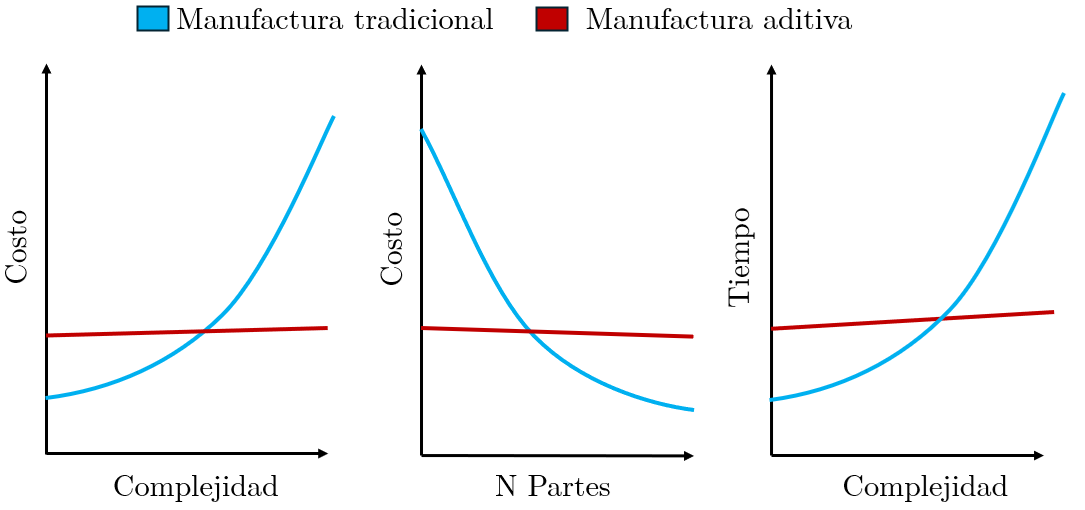
\includegraphics[width=0.9\linewidth]{imgs/grafsmm.png}
	\caption{Comparaciones entre procesos convencionales y de manufactura aditiva.}
	\label{grafsmm}
\end{figure}

La evolución del volumen de producción de un componente o producto define el punto de equilibrio en el que los sistemas flexibles de manufactura (como CNCs) dejan de ser competitivos frente a maquinaria altamente especializada. En lotes pequeños o medianos, la ausencia de conjuntos de herramientas y la capacidad de reconfiguración rápida de CNC y manufactura aditiva ofrecen tiempos de respuesta reducidos y bajos costos iniciales. Sin embargo, a medida que el tamaño del lote supera un umbral crítico, la inversión en moldes, troqueles o líneas automatizadas amortiza su alto coste inicial mediante ciclos unitarios extremadamente rápidos y costos marginales decrecientes.  

En consecuencia, la manufactura aditiva despliega su mayor ventaja competitiva en nichos de mercado caracterizados por:

\begin{itemize}
  \item \textbf{Producción on-demand} de piezas personalizadas (por ejempllo, prótesis y órtesis a medida), donde cada muestra requiere geometrías únicas.  
  \item \textbf{Componentes aeroespaciales} con topologías optimizadas para relación resistencia-peso y cavidades internas complejas.  
  \item \textbf{Herramientas de serie corta y prototipos funcionales} en proyectos de I+D, donde la flexibilidad de diseño y la velocidad de iteración priman sobre el coste unitario.  
  \item \textbf{Piezas de edición limitada} en sectores como automoción de alta gama o diseño industrial, donde el valor añadido justifica tiempos de fabricación superiores.
\end{itemize}  

Aunque la manufactura aditiva presenta ciertas restricciones para su producción industrial a gran escala, especialmente en términos de tiempos de ciclo y costo unitario, resulta una herramienta inigualable durante la fase de prototipado, razón principal para el nacimiento de estas tecnologías.

\subsection{Tipos de tecnologías}

Bajo la definición anterior, las familias generales de tecnologías de manufactura aditiva son:

\begin{itemize}
  \item \textbf{Vat photopolymerization:}  
    fotopolimerización selectiva de una resina líquida en un tanque mediante un haz de luz (láser o proyector). Cada capa se cura en la zona expuesta, obteniéndose piezas con alta resolución y excelente acabado superficial. Materiales típicos: resinas acrílicas, epóxicas o híbridas.

  \item \textbf{Material extrusion:}  
    extrusión de material termoplástico, cerámico, metálico (filamento o pasta) a través de una boquilla calentada. El cordón depositado se funde y solidifica capa a capa. Materiales típicos: PLA, ABS, Nylon, pastas cerámicas o compuestos cargados.

  \item \textbf{Material jetting:}  
    depositado por inyección de gotas de material (resinas, cerámicas, ceras o metales) a través de cabezales piezoeléctricos, seguido de fotopolimerización o fusión local. Permite impresión multi-material y gradientes de propiedades en una misma pieza.

  \item \textbf{Binder jetting:}  
    chorro de un aglomerante líquido sobre un lecho de polvo (polímero, metal o cerámico) para aglomerar selectivamente las zonas deseadas. Tras la impresión, la pieza en verde se cura o sinteriza para densificarla. Materiales típicos: acero, aluminio, arena de sílice, polvos cerámicos.

  \item \textbf{Powder bed fusion:}  
    fusión o sinterizado selectivo de un lecho de polvo mediante un láser o haz de electrones. El polvo sinterizado actúa de andamiaje, eliminando la necesidad de soportes. Materiales típicos: poliamidas, polietileno, aleaciones de aluminio, acero, titanio.

  \item \textbf{Direct energy deposition:}  
    alimentación simultánea de polvo o alambre con un haz de energía (láser, electrones, plasma) que funde el material en el punto de deposición. Ideal para reparaciones y recubrimientos de componentes metálicos. Materiales típicos: aceros inoxidables, aleaciones de titanio, superaleaciones.

  \item \textbf{Sheet lamination:}  
    unión de láminas de material (papel, polímero, metal o compuestos) mediante adhesivos, soldadura láser o ultrasonidos, y corte secuencial de cada capa para formar la geometría final. Materiales típicos: acero laminado, aluminio, papel tratado, polímeros.
\end{itemize}

Cada una de estas tecnologías de manufactura aditiva presenta atributos particulares que las hacen idóneas para aplicaciones específicas. La selección de la tecnología más adecuada debe fundamentarse en la combinación de parámetros como el tipo de material, la resolución requerida, el coste unitario y el volumen de producción.  

Gran parte de estas máquinas ha experimentado una evolución estructural análoga a la de los computadores: de voluminosos sistemas industriales, costosos y de manejo complejo, a una amplia oferta de modelos de escritorio, asequibles y de operación intuitiva. Esta transformación se ha materializado principalmente en las dos tecnologías aditivas más populares, extrusión y fotopolimerización en vat, impulsadas por el movimiento maker, el desarrollo de plataformas open-source y la diversificación de materiales compatibles.

\subsection{Slicer}

En el flujo de trabajo de fabricación aditiva, el software CAM incorpora un módulo slicer que segmenta el modelo 3D en $n$ planos horizontales (paralelos al eje $x-y$). Cada uno de estos cortes tiene un espesor igual al parámetro operativo de \textbf{altura de capa} y será la unidad básica que se apile durante la impresión para reconstruir la geometría del diseño.

La altura de capa es un parámetro crítico: define la resolución y la fidelidad geométrica de la pieza, y condiciona el tiempo total de fabricación. Una capa más delgada mejora el detalle superficial y la precisión dimensional, pero exige más pasadas de extrusión y prolonga el tiempo de impresión. En cambio, capas más gruesas aceleran el proceso a costa de perder definición en detalles finos.

Sobre cada sección transversal generada, el slicer traza la trayectoria de la herramienta (toolpath) y genera el código G correspondiente en función del resto de parámetros operativos a configurar en el CAM.

El archivo que se importa al slicer rara vez conserva el formato nativo del CAD (por ejemplo, STEP o IGES); en su lugar se convierte la superficie del modelo en una malla poligonal que la aproxima, normalmente mediante un archivo con extensión .stl. En este formato, la geometría 3D se tesela en triángulos: las curvas y detalles se aproximan con facetas planas, pero se pierde por completo la información volumétrica interna (materiales, estructuras huecas o sólidos). El acrónimo STL se interpreta habitualmente como Stereolithography, Standard Tessellation Language o Standard Triangle Language. 

El grado de refinamiento de esa malla condiciona la fidelidad entre el diseño original y lo que realmente procesa el slicer: una malla demasiado gruesa produce polígonos (facetas) visibles, mientras que una demasiado densa no mejora la calidad de impresión, pues la impresora tiene una resolución limitada. Es clave elegir un nivel de detalle óptimo que equilibre precisión y eficiencia computacional.

Este archivo sólo describe la envolvente externa de la pieza; no incluye información sobre su volumen o espesores interiores. Estas características serán definidas mediante los parámetros del CAM a utilizar.

\section{Impresión 3D por extrusión}

\subsection{Modelado por deposición fundida}

Esta tecnología de manufactura se basa en la deposición controlada de material a través de una boquilla dispensadora. Su aplicación más común es la impresión con filamento termoplástico: un motor impulsa el hilo hacia un módulo de calentamiento que aplica un perfil térmico preciso. De este modo, el polímero permanece rígido durante el avance y se ablanda al atravesar la zona caliente, alcanzando la viscosidad óptima para su extrusión controlada.

Una vez depositado el material, este se solidifica casi de inmediato en el lugar donde fue extruido (idealmente), enfriándose y recuperando rigidez. Esto se repite capa a capa hasta construir la geometría deseada.

La impresora emplea una arquitectura cinemática tridimensional, diseñada para mover el cabezal sin necesidad de fuerzas elevadas, más allá de las requeridas para vencer su propia inercia. La masa móvil depende de la posición del motor de extrusión, que puede situarse dentro del cabezal (\textbf{extrusión directa}) o en un soporte externo (\textbf{sistema Bowden}).

El sistema Bowden reduce significativamente la masa del cabezal, disminuye la inercia y permite mayores aceleraciones con menos vibraciones. En cambio, el extrusor directo, al llevar el motor integrado en el cabezal, minimiza el roce y la deformación del filamento, mejorando la calidad de la extrusión, especialmente con materiales flexibles.

El cabezal cuenta con diversas componentes, encargadas de dirigir el filamento y otorgar el gradiente térmico:

\begin{itemize}
  \item \textbf{Calefactor y termocupla}: Este par permite aplicar y mantener con precisión el perfil térmico necesario para fundir el filamento.

  \item \textbf{Disipador}: bloque de aluminio con aletas diseñado para extraer el calor en el cabezal y evitar el paso de este hacia la zona fría. Garantiza que el filamento se mantenga rígido hasta llegar al bloque calefactor, previniendo atascos.

  \item \textbf{Ventilador}: montado sobre el disipador, impulsa aire en las aletas para optimizar la extracción de calor. 

  \item \textbf{Ventilador de capas}: enfoca un flujo de aire directo sobre la pieza impresa, acelerando la solidificación del plástico extruido. 

  \item \textbf{Boquilla}: punta de latón, acero o acero endurecido con un orificio calibrado (generalmente de 0.4 mm). Controla el flujo de material fundido y define la resolución, el ancho de línea y el volumen de extrusión de cada capa.
\end{itemize}

Esta técnica de impresión es actualmente la más popular, pues la simplicidad de la máquina y el costo de los materiales permite que existan modelos de escritorio de alrededor de unos cien dólares.

En la impresión FDM, el plástico se deposita sobre una \textbf{plataforma o cama}, que puede ser fija o móvil según la arquitectura cinemática de la impresora. La adhesión de la primera capa es crítica, pues de ella depende la estabilidad de todo el conjunto; el fallo más habitual es el despegue de la pieza durante la impresión. Para optimizar el contacto, la boquilla debe quedar perfectamente perpendicular a la superficie de la cama. Esta nivelación se logra mediante calibración manual, sistemas de nivelación automática o ajustes adaptativos por sensores, según el modelo de impresora. 

La adhesión del plástico ocurre al fluir el plástico caliente entre los micro relieves de la cama, anclándose mecánicamente. Además, esta adhesión podría ser favorecida cuando existe afinidad química o polar entre el polímero y el material de la base. La plataforma de impresión puede presentar distintas rugosidades: una superficie texturizada favorece la adherencia del filamento, pero está sujeta a desgaste, mientras que el vidrio liso proporciona un acabado más pulido y durabilidad, pero es más difícil la adhesión.

El despegue de la pieza suele originarse por \textbf{warping}, un fenómeno en el que los gradientes térmicos durante el enfriamiento generan tensiones internas que deforman y curvan los bordes, separándolos de la cama. Para contrarrestar este efecto, la plataforma se calienta hasta una temperatura cercana al punto de transición vítrea del polímero. Así, la pieza se enfría de forma más gradual y permanece más flexible, reduciendo las tensiones por contracción térmica. Algunos modelos de impresoras presentan un \textbf{ambiente cerrado}, el cual puede incluso contar con control de temperatura, controlando mejor los gradientes térmicos generados durante el proceso.

Al elegir un material para impresión FDM, resulta fundamental entonces que su \textbf{coeficiente de dilatación térmica} sea bajo. Esta característica minimiza el warping y refuerza la precisión dimensional al reducir la variación de volumen durante el enfriamiento. Por ello, el coeficiente de dilatación es un parámetro clave para la facilidad de impresión o \textbf{imprimibilidad} de un polímero. Existen otras propiedades mecánicas que influyen en el proceso, pero suelen requerir compromisos, cada una tiene una ventana óptima de funcionamiento en lugar de un valor extremo universal.

\begin{table}[h]
  \centering
  \footnotesize
  \begin{tabular}{|p{3cm}|p{5cm}|p{5cm}|}
    \hline
    \textbf{Propiedad} & \textbf{Muy baja} & \textbf{Muy alta} \\
    \hline
    Coeficiente de dilatación térmica (\(\alpha\)) 
      & Contracción casi nula y mínima deformación térmica 
      & Elevadas tensiones internas, warping pronunciado y despegue de bordes \\
    \hline
    Difusividad térmica 
      & Gradientes térmicos marcados, warping localizado y mala unión intercapas 
      & Enfriamiento demasiado rápido, fusión insuficiente entre capas \\
    \hline
    Viscosidad fundida 
      & Filamento excesivamente fluido: colapso de voladizos y goteo constante 
      & Extrusión irregular, obstrucciones y falta de flujo uniforme \\
    \hline
    Adhesión intercapas 
      & Delaminación, baja resistencia mecánica y capas sueltas 
      & Sobrellenado, pérdida de detalle en bordes y posibles deformaciones \\
    \hline
    Elongación a rotura (\(\%\)) 
      & Piezas frágiles, fisuras y roturas en puentes y voladizos 
      & Deformaciones postimpresión, tendencia a serpentear o estirarse bajo peso \\
    \hline
    Módulo de elasticidad (\(E\)) 
      & Capas se arquean bajo su propio peso y geometría inestable 
      & Estructuras rígidas y quebradizas, propagación rápida de grietas \\
    \hline
    Temperatura de transición vítrea (\(T_g\)) 
      & Material blando en impresión: deformaciones y colapso de detalles 
      & Difícil soldado de capas posteriores, requiere camas muy calientes \\
    \hline
  \end{tabular}
  \caption{Propiedades termomecánicas críticas para la imprimibilidad en FDM.}
  \label{tab:propiedades_fdm}
\end{table}

Una limitante en los sistemas de impresión suele ser la temperatura de fusión del material, pues temperaturas muy altas implican un mejor diseño y selección en las componentes que podrían verse degradadas por el flujo de calor. Típicamente, los materiales que presentan mejores propiedades mecánicas tienden a ser imprimidos a temperaturas más altas, requiriendo más prestaciones en la máquina. Los materiales tradicionales básicos se imprimen cerca de los 200.

Los filamentos para impresión 3D se suministran habitualmente en carretes de 1 kg con diámetros estándar de 1,75 mm (también existen versiones de 2,85 mm). Se envasan al vacío junto a paquetes de gel de sílice para controlar la humedad, ya que la mayoría de los polímeros son higroscópicos. Por ello, resulta crucial que un material de impresión muestre baja higroscopicidad: el agua absorbida no solo puede alterar sus propiedades mecánicas y térmicas, sino que al vaporizarse durante la extrusión provoca burbujas y discontinuidades en el flujo, comprometiendo la calidad y la fiabilidad de cada pieza.

\begin{table}[h]
  \centering
  \small
  \begin{tabular}{|l|c|p{5cm}|p{5cm}|}
    \hline
    \textbf{Material}    & \textbf{T\textsubscript{e} °C} & \textbf{Ventajas}                          & \textbf{Limitaciones}                             \\
    \hline
    PLA                  & 180–220                           & Fácil de imprimir, biodegradable, baja deformación              & Fragilidad y baja resistencia térmica               \\
    \hline
    ABS                  & 220–260                          & Buena resistencia mecánica y térmica                           & Warping pronunciado; requiere cama caliente y recinto     \\
    \hline
    PETG                 & 230–250                          & Excelente adhesión intercapas; resistencia química             & Stringing; definición moderada en detalles finos       \\
    \hline
    TPU                  & 210–240                         & Alta flexibilidad y resistencia al impacto                     & Extrusión y retracción complejas; velocidades bajas        \\
    \hline
    Nylon (PA)           & 240–260                        & Gran tenacidad y resistencia al desgaste                       & Higroscopicidad alta; warping y cámara cerrada requerida   \\
    \hline
    PC                   & 260–300                          & Muy alta resistencia mecánica y térmica                        & Difícil adhesión y manejo; necesita cama muy caliente      \\
    \hline
    ASA                  & 240–260                           & Resistente a UV e intemperie; similar al ABS sin amarilleo     & Requiere recinto cerrado; warping moderado                 \\
    \hline
    PVA        & 180–220                           & Soluble en agua para soportes complejos                       & Muy higroscópico; vida útil corta                          \\
    \hline
  \end{tabular}
  \caption{Materiales comunes en impresión FDM: rango de temperatura de extrusión, ventajas y limitaciones.}
  \label{tab:materiales_fdm}
\end{table}

\subsection{Morfología de una impresión FDM}

Si bien la tecnología de fabricación por deposición fundida (FDM) admite múltiples estrategias de deposición, el método convencional consiste en generar la pieza de forma estratificada: el extrusor deposita cada capa sobre el plano XY y, al completarse, el sistema aumenta su posición en el eje Z para continuar la construcción hasta finalizar la pieza. Esta corresponde a una estrategia \textbf{planar}.

Una estrategia \textbf{no planar} extiende la deposición de filamento más allá de las capas horizontales, trazando trayectorias tridimensionales curvadas que se adaptan con precisión a la geometría del modelo y preservan el detalle que habitualmente se pierde por la altura de capa. No obstante, esta técnica demanda un cálculo de toolpaths mucho más complejo y algoritmos de slicing adaptativos, y requiere planificar con cuidado los movimientos para evitar colisiones entre el extrusor y la pieza.

En la estrategia planar estándar, el extrusor dibuja primero los perímetros o paredes, que definen la silueta y las dimensiones finales de la pieza. A continuación deposita material en el interior, cuya estrategia varía según la ubicación de la capa dentro del volumen. Entre las características más notorias del proceso FDM se encuentra la rugosidad superficial inherente, derivada de la deposición capa a capa del material fundido.

Las capas iniciales (base) y finales (tapas superior e inferior) se imprimen sólidas para garantizar rigidez y un acabado uniforme. Entre ellas, las capas intermedias emplean un patrón de relleno (infill) de densidad controlada: este entramado interno aporta soporte a las paredes y capas superiores, reduce el consumo de material y acorta los tiempos de impresión sin comprometer críticamente la rigidez general. Este paradigma proviene del prototipado rápido, en el que la forma externa y la velocidad de fabricación eran prioritarias.

De este modo, una pieza impresa se organiza en paredes (shells), relleno (infill) y tapas superior e inferior (top y bottom), aunque el proceso puede requerir estructuras auxiliares. En FDM se asume que cada capa descansa sobre la anterior, pero cuando aparece un voladizo, es decir, un tramo suspendido más allá de lo que admite la viscosidad del plástico fundido, el material tiende a colapsar, provocando imprecisiones geométricas o incluso interrumpiendo la impresión. Para evitarlo, el software CAM puede generar automáticamente \textbf{soportes} que sostienen estas zonas en voladizo, garantizando la continuidad y la precisión dimensional del proceso.

Otras estructuras auxiliares aportan a la adhesión de la primera capa, como por ejemplo:

\begin{itemize}
  \item \textbf{Brim}: líneas adicionales adjuntas al perímetro de la primera capa que amplían la superficie de contacto y reducen el warping de los bordes.  
  \item \textbf{Raft}: rejilla sacrificial impresa bajo toda la pieza que corrige desniveles, atenúa gradientes térmicos y facilita el desmoldeo posterior.  
  \item \textbf{Skirt}: contorno exterior impreso en vacío antes de la pieza, usado para cebar el flujo y validar temperatura y presión sin afectar la adhesión directa.  
\end{itemize}

\subsection{Comportamiento mecánico de piezas impresas}

Por lo anterior, la forma en que se generan las piezas mediante impresión FDM da lugar a estructuras inherentemente no homogéneas, y por lo tanto, anisotrópicas. Como se observa en la Figura \ref{segmens}, que muestra un corte transversal de una pieza impresa, es evidente que existen diferencias tanto en el área de contacto entre los segmentos de material extruido como en la calidad de la unión entre ellos, la cual depende de la difusión de cadenas poliméricas entre segmentos adyacentes.

La efectividad de esta soldadura intersegmental depende en gran medida de que la temperatura en la zona de unión se mantenga dentro de un rango adecuado durante un tiempo mínimo. Esta condición térmica es la que permite la movilidad molecular necesaria para que ocurra la difusión de cadenas entre segmentos depositados en momentos distintos. Sin embargo, temperaturas excesivamente altas pueden comprometer la integridad de la pieza, ya que el material puede entrar en un régimen de flujo viscoso, afectando negativamente la geometría y las tolerancias dimensionales.

Desde un punto de vista mecánico, el escenario más favorable se presenta cuando una fuerza externa se aplica en dirección paralela a los segmentos de material más extensos (por ejemplo, a lo largo de una línea de extrusión continua). En este caso, el esfuerzo se distribuye a lo largo de una trayectoria donde el material ha sido depositado de manera continua y homogénea, presentando una unión interna más sólida.

Un escenario menos favorable ocurre cuando la carga se aplica en dirección perpendicular a la orientación principal de los filamentos. En este caso, el área bajo tracción corresponde a las uniones entre segmentos que fueron extruidos en momentos distintos, lo que puede implicar diferencias térmicas significativas durante su deposición y, en consecuencia, una menor difusión entre cadenas y una unión más débil.

Finalmente, el escenario más crítico desde el punto de vista estructural es aquel en el que la carga se aplica en dirección normal al plano de las capas (es decir, a lo largo del eje Z), o cuando se trata de una fuerza de corte interlaminar. En este caso, la resistencia mecánica depende casi exclusivamente de la adherencia entre capas sucesivas, las cuales se enfrían parcialmente antes de recibir la siguiente capa, lo que reduce notablemente la capacidad de difusión entre cadenas y genera zonas de alta vulnerabilidad.

Cabe señalar que el fenómeno descrito es aún más complejo, ya que, como se mencionó en la sección anterior, una impresión FDM estándar está compuesta por distintas secciones funcionales, cada una de las cuales se imprime con patrones y estrategias particulares. En consecuencia, el comportamiento mecánico y estructural final de la pieza estará determinado por los parámetros de impresión configurados en el slicer. A su vez, dichas configuraciones deben estar alineadas con las capacidades y limitaciones de la máquina específica con la que se realizará la fabricación, incluyendo aspectos como la precisión del extrusor, el control térmico y el sistema de movimiento.

El uso principal de la tecnología FDM se centra en el prototipado rápido, por lo que en muchos casos las propiedades mecánicas de las piezas generadas no son un factor crítico. Sin embargo, cuando se busca emplearlas en aplicaciones funcionales, surgen limitaciones importantes. Las piezas impresas en 3D mediante FDM presentan una notable sensibilidad térmica y su comportamiento mecánico es difícil de predecir en comparación con materiales de propiedades homogéneas. Esto se debe a que su resistencia está fuertemente influenciada por las condiciones locales de impresión, como la orientación de las capas, la calidad de adhesión entre filamentos y los acabados de borde. Como resultado, las piezas impresas suelen exhibir una resistencia mecánica inferior frente a sus equivalentes fabricados por inyección.

Además, los filamentos utilizados en impresión FDM no están compuestos exclusivamente del polímero base, sino que incluyen una variedad de aditivos y cargas (fillers) destinados a mejorar el proceso de extrusión, la estabilidad térmica y la calidad superficial. Estos compuestos pueden diferir significativamente de los utilizados en plásticos inyectados, lo que también contribuye a las diferencias en comportamiento estructural y desempeño final.

\subsection{Parámetros operativos}

Los parámetros de impresión deben definirse en función del objetivo específico de la pieza, lo que generalmente implica un compromiso (trade-off) entre tiempo de fabricación, calidad superficial y resistencia mecánica. Por ejemplo, una menor altura de capa permite una mayor fidelidad con el modelo 3D y mejor acabado superficial, pero incrementa significativamente el tiempo total de impresión. De manera similar, reducir el porcentaje de relleno acelera el proceso y ahorra material, pero también disminuye el soporte estructural interno, aumentando el riesgo de fallas mecánicas.

Entre estos parámetros, la velocidad de impresión requiere un análisis particularmente cuidadoso debido a su impacto directo en la calidad y funcionalidad de la pieza.

En general, velocidades de impresión bajas tienden a producir mejores resultados, ya que permiten una deposición más precisa del material y una mejor adhesión entre capas. Por el contrario, al incrementar la velocidad, se introducen diversos problemas: el cabezal puede generar vibraciones mecánicas que afectan la precisión dimensional y el acabado superficial, y se incrementan las demandas sobre el sistema de extrusión, como el torque del motor, el flujo térmico en el cabezal y la capacidad del sistema de enfriamiento.

Además, velocidades excesivamente altas pueden provocar una acumulación de calor en zonas localizadas, ya que el filamento recién depositado no tiene tiempo suficiente para enfriarse adecuadamente. Esto puede llevar a que el material se mantenga en un estado semifundido durante más tiempo del deseado, volviéndose susceptible a deformaciones térmicas. Estas deformaciones pueden originarse por su propio peso, la acción del ventilador, o incluso el contacto indirecto con el cabezal en movimiento, ya que el filamento aún viscoso en la boquilla puede arrastrar o desplazar partes parcialmente solidificadas de la pieza.

Este fenómeno es particularmente crítico en piezas con detalles finos o geometrías pequeñas, donde el tiempo de exposición térmica acumulada es mayor y el riesgo de distorsión se incrementa notablemente.

Por esta razón, las zonas superficiales de la pieza suelen imprimirse a menor velocidad, con el fin de asegurar una mayor precisión dimensional y una mejor calidad superficial. En contraste, las secciones internas, que cumplen principalmente una función de soporte estructural, se imprimen a velocidades más altas, ya que no afectan directamente la apariencia ni la precisión de la pieza final.

En particular, la primera capa se imprime significativamente más lenta que el resto del modelo. Esta estrategia busca garantizar una correcta adherencia a la cama de impresión, lo cual es fundamental para evitar desplazamientos, deformaciones o desprendimientos durante el proceso. Recordemos que cualquier distorsión en esta capa puede impedir la impresión correcta de las capas sucesivas.

En un proceso de impresión 3D, existe una gran cantidad de variables que deben ser definidas para garantizar resultados óptimos. No obstante, la mayoría de los valores funcionales predeterminados suelen estar preconfigurados en el software CAM (slicer) según el modelo específico de impresora y el tipo de material seleccionado, lo que facilita la configuración inicial.

Estos parámetros pueden agruparse en tres grandes categorías: estructurales, de proceso y de máquina. Esta clasificación también refleja, en gran medida, su importancia relativa en la calidad y éxito del proceso de impresión. 

Los parámetros estructurales (Cuadro \ref{tab:param-estructurales}) son aquellos que definen la morfología interna y externa de la pieza, incluyendo aspectos como el número de paredes (o espesor), el patrón y porcentaje de relleno, o la altura de capa. Son los parámetros más comúnmente ajustados al momento de optimizar el balance entre tiempo de impresión, calidad superficial y resistencia mecánica.

\begin{table}[ht]
  \centering
  \caption{Ejemplos de parámetros estructurales y valores típicos en impresoras de escritorio}
  \label{tab:param-estructurales}
  \begin{tabular}{@{} l c c @{}}
    \toprule
    Parámetro                   & Acrónimo       & Valor típico     \\
    \midrule
    Densidad de relleno        & $i_{\%}$     &     $\mathrm{10-20}$ $\%$\\
    Espesor de pared            & $t_{p}$        &   $\mathrm{0.8}\,mm$  \\
    Espesor de tapa superior          & $t_{t}$ & $\mathrm{0.5-1}\,mm$\\
    Espesor de tapa inferior            & $t_{b}$ & $\mathrm{0.5-1}\, mm$\\
    Altura de capa           & $h_{l}$            &  $\mathrm{0.1-0.3}\, mm$    \\
    \bottomrule
  \end{tabular}
\end{table}

Por otro lado, los parámetros de proceso (Cuadro \ref{tab:param-proceso}) están estrechamente relacionados con las propiedades térmicas y físicas del material utilizado. Variables como la temperatura de extrusión, la temperatura de la cama o la velocidad de enfriamiento deben ser cuidadosamente ajustadas según el tipo de polímero, ya que variaciones inadecuadas pueden comprometer la integridad estructural de la pieza o incluso impedir su correcta fabricación.

\begin{table}[ht]
  \centering
  \caption{Ejemplos de parámetros del proceso y valores típicos en impresoras de escritorio}
  \label{tab:param-proceso}
  \begin{tabular}{@{} l c c @{}}
    \toprule
    Parámetro                         & Acrónimo  & Valor típico  \\
    \midrule
    Velocidad de impresión            & $V_{f}$ &    $\mathrm{30-60}\,mm/s$  \\
    Temperatura de extrusión          & $T_{e}$  &    $\mathrm{190-220}\, \si{\celsius}$\\
    Temperatura de plataforma         & $T_{b}$   & $\mathrm{40-60}\, \si{\celsius}$ \\
    Porcentaje de ventilación         & $v_{\%}$ & $\mathrm{0-100}$ $\%$\\
    \bottomrule
  \end{tabular}
\end{table}

Finalmente, los parámetros de la máquina (Cuadro \ref{tab:param-hardware}) están vinculados a las características físicas del hardware, como el diámetro de la boquilla, el tipo de extrusor o la geometría del cabezal de impresión. Estos valores no deberían ser modificados salvo que se realicen cambios en la configuración física del equipo, ya que influyen directamente en la capacidad de extrusión y en la calidad final del proceso.

\begin{table}[ht]
  \centering
  \caption{Ejemplos de parámetros de hardware y valores típicos en impresoras de escritorio}
  \label{tab:param-hardware}
  \begin{tabular}{@{} l c c@{}}
    \toprule
    Parámetro                                   & Acrónimo & Valor típico  \\
    \midrule
    Diámetro de boquilla                        & $d_{\mathrm{noz}}$ &  $\mathrm{0.2-0.8}\,mm$ \\
    Diámetro de filamento                       & $d_{\mathrm{fil}}$ & $\mathrm{1.75}\,mm$ \\
    Volumen de impresión X (ancho)              & $L_{x}$   & $\mathrm{200-250}\,mm$\\
    Volumen de impresión Y (profundidad)        & $L_{y}$   & $\mathrm{200-250}\,mm$ \\
    Volumen de impresión Z (altura)             & $L_{z}$   & $\mathrm{200-250}\,mm$ \\
    \bottomrule
  \end{tabular}
\end{table}

\subsection{Procesamiento en CAM}

El éxito de una impresión FDM no solo depende de los valores de los parámetros en el slicer, sino también de cómo se dispone el objeto dentro del volumen de impresión. La orientación elegida influye en la adhesión a la cama, la generación de soportes, el tiempo total de fabricación, la resistencia mecánica de la pieza y la calidad superficial del modelo.

La inclinación del modelo determina dónde y cuántos soportes serán necesarios. Idealmente debe minimizarse la cantidad y la altura de las estructuras de soporte para reducir el consumo de material y el tiempo de impresión, así como para evitar daños en la superficie al retirarlos. Cuando resulte imprescindible emplear soportes, conviene ubicarlos en zonas poco críticas para la unión de partes, la estética o el postprocesado, de modo que su extracción sea más sencilla y afecte lo menos posible al acabado final.

La orientación del objeto también modifica su altura en el eje Z, lo que repercute directamente en el número de capas y, por tanto, en el tiempo de impresión. Al rotar o inclinar el modelo conviene evaluar el efecto en la duración del proceso, ya que una altura más corta en Z suele suponer una reducción significativa del tiempo de fabricación.

Para asegurar una buena adhesión de la primera capa, es recomendable apoyar la cara más plana y amplia del modelo contra la plataforma de impresión. También es fundamental controlar los parámetros térmicos, ya que una mayor área de contacto puede aumentar el riesgo de warping si la máquina no está correctamente calibrada.

Las piezas fabricadas por FDM son anisotrópicas: la unión intercapas (dirección Z) es intrínsecamente menos resistente que la propia capa (plano XY). Por ello, al orientar la pieza conviene alinear las capas con las direcciones de carga para evitar esfuerzos de corte o delaminación que comprometan la resistencia mecánica del objeto.

La discretización de superficies curvas mediante capas planas genera un efecto escalonado. Para minimizar este “stepping” en zonas con curvaturas pronunciadas, es preferible orientar la geometría de manera que las curvas principales queden lo más paralelas posible al plano XY, mejorando así la calidad superficial sin necesidad de aumentar excesivamente el número de capas.

Con la orientación definida se procede a configurar los parámetros en el CAM, definiendo además si es que dada la pieza y lo deseado se quieren soportes o estructuras extra de adhesión a la cama. El software entregará una simulación del proceso y de las rutas de fabricación. 

La cantidad de filamento a extruir ($E$) en cada segmento del cuerpo se calcula mediante una conservación de volumen entre lo que entra (filamento) y lo que se quiere construir (segmento):

\begin{equation}
	V_{segmento}=V_{filamento}\implies l_{s}h_{l}d_{noz}=\frac{d_{fil}^{2}\pi}{4}E\implies E= \frac{4 l_{s}h_{l}d_{noz}}{d_{fil}^{2} \pi}
\end{equation}

Asumiendo un área aproximadamente rectangular para el segmento.

\subsection{Defectos típicos en FDM}

Fuera de la porosidad, resistencia intercapa y rugosidad intrínseca de las piezas fabricadas mediante el proceso, existen diversos defectos en la impresión 3D que pueden originarse tanto por el desgaste de componentes  del hardware como por una configuración inadecuada de los parámetros de proceso. 

Entre los más comunes están el \textit{stringing} y el \textit{oozing}, que se manifiestan cuando el filamento fundido fluye de forma indeseada durante los desplazamientos del extrusor. El stringing genera finos hilos de plástico entre zonas no contiguas de la pieza, mientras que el oozing, o goteo, es la exudación continua de material cuando la extrusión debería estar detenida. Ambos fenómenos se agravan si la temperatura de la boquilla es demasiado alta y la viscosidad del polímero disminuye, pues el material fluye por gravedad o presión residual.

Para mitigar estos efectos, la retracción de filamento es esencial. Al retroceder el filamento una distancia calibrada y a una velocidad adecuada, se crea una presión negativa en la cámara de fusión que impide la fuga de material. Los parámetros para la retracción también son ajustables en el software CAM.

La propia geometría de la pieza puede desencadenar defectos puntuales, como el sobrecalentamiento de detalles altos y delgados, donde la rigidez es podría ser muy baja. Este problema de refrigeración tiene múltiples soluciones, que también pueden presentarse como un ajuste más de parámetros en el CAM, por ejemplo, modificando el tiempo mínimo por capa.

El parámetro \textit{flow} ajusta el caudal de filamento mediante un porcentaje sobre el valor nominal, actuando como un multiplicador del volumen extruido. En la Figura X se observan dos defectos contrapuestos: un \textit{flow} insuficiente provoca huecos y capas discontinuas, mientras que un exceso de flujo deriva en protuberancias y acumulaciones de material. Aunque es posible reducir ambos efectos modificando directamente el \textit{flow}, esta práctica solo enmascara el síntoma, ya que la causa real puede residir en variaciones del diámetro del filamento, una temperatura de boquilla mal calibrada, sobrepresión en el sistema de alimentación o errores de configuración.

El ajuste del caudal puede ser útil para compensar los efectos elásticos de la extrusión ocasionados por el \textbf{die swelling}, un fenómeno directamente ligado a la velocidad de extrusión: a mayores velocidades, la recuperación elástica del polímero al liberarse de la presión en la boquilla es más intensa, ensanchando el segmento por encima del diámetro nominal.
Este sobredimensionamiento se manifiesta como solapamientos en esquinas y en la uniformidad de las paredes. 

\subsection{Otras tecnologías de deposición}

\subsubsection{Impresión FDM con pellets}

Los polímeros como materiales de ingeniería se obtienen mediante procesos de síntesis que involucran varias etapas, culminando en la conformación de la materia prima en formatos comercializables desde pellets. En el caso particular de la impresión 3D, el filamento es un producto derivado de estos pellets, y su fabricación implica procesos adicionales de extrusión, calibración y embobinado, lo que le confiere un mayor valor agregado.

Sin embargo, en aplicaciones industriales y de gran formato, han surgido impresoras FDM capaces de trabajar directamente con pellets impulsados por un tornillo de extrusión (similar a las máquinas de inyección), eliminando la necesidad de convertir previamente el material en filamento. Este enfoque ofrece una reducción significativa en los costos de material, ya que los pellets son una forma comercial estándar y económica, disponible a granel, y sin los procesos intermedios asociados al filamento.

Este tipo de impresión es especialmente útil en impresoras de gran volumen, donde el uso de filamento puede resultar ineficiente debido a la necesidad de recambios frecuentes de carretes. En cambio, las máquinas que utilizan pellets incorporan tolvas de gran capacidad para la alimentación del material o incluso sistemas de alimentación continua, lo que permite una operación prolongada y más autónoma, así como un mayor flujo y diámetros de boquilla. Además, los pellets empleados no requieren una granulometría estricta, lo que aumenta la flexibilidad en el tipo de material utilizado.

Una ventaja adicional de esta tecnología es la posibilidad de personalizar el material, ya que pueden mezclarse distintos tipos de pellets o incorporar aditivos durante la alimentación, permitiendo modificar propiedades térmicas, mecánicas o estéticas del polímero.  

No obstante, este método también presenta desafíos importantes. A diferencia del filamento, cuya forma cilíndrica garantiza una extrusión continua y uniforme, la extrusión directa de pellets puede ser más inestable y está fuertemente influenciada por el diseño del tornillo sinfín, responsable de transportar y fundir el material. La eficiencia, homogeneidad del flujo y calidad de impresión final dependen críticamente de este componente, lo que añade complejidad al diseño y operación de las máquinas.

Por esto, no es sencillo definir los pasos del motor del tornillo de extrusión, pues a pesar de que existe un cálculo directo del volumen de extrusión nominal, dependerá de las fluctuaciones de pellets, la velocidad y la elasticidad. Aquí entra en juego el parámetro de flow, calibrándolo para cada material.

\subsubsection{Impresión de pastas}

Un sistema de extrusión análogo al de plástico fundido permite imprimir pastas cerámicas en frío, como arcillas o gredas, sin necesidad de un sistema calefactor. Estas suspensiones se preparan ajustando la proporción de agua y aditivos (defloculantes, plastificantes) para lograr un comportamiento reológico que combine fácil flujo bajo presión con cohesión inmediata tras la deposición, de modo que cada cordón mantenga su forma y resista el peso de las capas superiores.

El suministro de material suele ser a través de un estanque donde actúa un émbolo motorizado o una línea de aire comprimido. Bajo presión neumática o mediante un pistón de avance controlado, la pasta se impulsa hasta el cabezal, donde puede encontrarse un tornillo sinfín de precisión que ajusta el caudal real de extrusión. Este arreglo ofrece un control fino del volumen depositado, minimiza la pulsación y permite variar el grosor de línea al cambiar la velocidad de rotación o la presión de alimentación.

Tras la impresión, las piezas cerámicas requieren un postprocesado riguroso. Primero se someten a un secado lento y controlado para evitar grietas o deformaciones por gradientes de humedad. A continuación, pasan a un horno de cocción con un programa de temperatura escalonado, que consolida la estructura, optimiza la densidad y controla la microestructura del material según las propiedades mecánicas y estéticas deseadas.

Bajo este mismo principio es que se imprimen grandes estructuras como casas, usando concretos y morteros especializados, así como grandes brazos robóticos para dar con la escala del proyecto.

\subsubsection{Impresión liquid-on-liquid}

En la impresión líquido–sobre–líquido, el cabezal deposita el material directamente en un volumen de soporte líquido. Este medio puede ser un fluido de comportamiento viscoso no newtoniano, una suspensión densamente cargada o un líquido inmiscible, y su función principal es mantener la forma durante la deposición sin necesidad de estructuras auxiliares sólidas.

Existen al menos tres variantes de esta técnica, dependiendo de la relación funcional entre el material impreso y el líquido de soporte. En la modalidad más extendida, la impresión constituye la pieza final y el medio líquido se retira posteriormente mediante decantación, lavado o centrifugado, seguido por un proceso de curado o secado. Una segunda variante invierte esta lógica: el material impreso actúa como un sacrificado que se elimina al final, mientras que el líquido se solidifica y forma parte del objeto final, como ocurre en la fabricación de canales encapsulados. En una tercera modalidad, tanto el líquido como el material impreso se conservan, configurando estructuras multicomponente con funcionalidades diferenciadas, como en sensores blandos.

Una de las aplicaciones más relevantes de esta técnica es la bioimpresión, un proceso de fabricación aditiva orientado a la deposición precisa de materiales biocompatibles, células vivas y factores de crecimiento para construir estructuras funcionales, como tejidos o andamios celulares. La impresión líquido–sobre–líquido resulta especialmente adecuada en este contexto, ya que permite mantener condiciones de baja tensión mecánica durante la deposición y evita la deformación o colapso de geometrías frágiles. Además, la compatibilidad del medio de soporte con soluciones acuosas y matrices extracelulares facilita la conservación de la viabilidad celular, así como la impresión directa en ambientes biológicamente activos.

Para que este proceso sea físicamente viable, deben cumplirse ciertas condiciones: la densidad del medio y del material impreso deben estar equilibradas para evitar flotación o sedimentación relativa, y deben evitarse interacciones que lleven a la formación de agregados o coalescencia entre cordones. Además, el medio debe ofrecer una resistencia suficiente al flujo para sostener la geometría durante la deposición, pero permitir el desplazamiento del cabezal sin perturbaciones significativas.

 
\section{Impresión 3D por fotopolimerización}

\subsection{Fotopolimerización}

La fotopolimerización es una reacción de química en la que monómeros y oligómeros se transforman en una red tridimensional por la acción de luz, normalmente en el rango de 365–405 nm. El proceso arranca cuando un fotón incide sobre un fotoiniciador presente en la mezcla, generando radicales libres. Estos transforman enlaces dobles en los monómeros a simples activos, iniciando reacciones en cadena que alargan y entrecruzan las cadenas poliméricas hasta \textbf{curar} el líquido en un sólido termoestable.

La densidad de entrecruzamiento y, por tanto, las propiedades mecánicas y dimensionales finales dependen de la dosis de energía (intensidad y tiempo de exposición), de la concentración de fotoiniciador y de la profundidad de penetración de la luz en el material. Un curado excesivo puede inducir tensiones internas y contracción volumétrica, mientras que una exposición insuficiente deja zonas sin polimerizar, con menor resistencia y rugosidad superficial. Una forma de estimar el tamaño de la zona en fotopolimerización puede ser mediante la ecuación de Jacobs:

\begin{equation}
	D_{\mathrm{curado}} \;=\; 2\,D_{p}\,\ln\!\Bigl(\frac{P\,t}{A\,E_{c}}\Bigr)
\end{equation}

donde:

\begin{description}
	\item[$D_{\mathrm{curado}}$] Diámetro de la zona polimerizada (misma unidad que $D_{p}$, por ejemplo mm).
	\item[$D_{p}$] Profundidad de penetración de la luz en el fotopolímero (mm).
	\item[$P$] Potencia de la fuente luminosa sobre el área irradiada (W).
	\item[$t$] Tiempo de exposición al haz de luz (s).
	\item[$A$] Área efectiva del haz o región iluminada (cm$^2$).
	\item[$E_{c}$] Dosis crítica mínima necesaria para iniciar la polimerización (J/cm$^2$).
\end{description}


\subsection{Estereolitografía}

La estereolitografía (SLA) fue la primera tecnología de impresión 3D patentada. Su funcionamiento se basa en la solidificación de resinas fotosensibles mediante irradiación láser UV, o fotopolimerización. El término procede del griego stereo (sólido), lithos (piedra) y graphia (escritura), es decir, escritura de sólidos.

La arquitectura clásica de una impresora SLA se ilustra en la Figura. Está formada por un tanque de resina líquida, una plataforma móvil en el eje Z y un sistema de escaneo láser (galvanómetro) que dirige el haz UV sobre la superficie del líquido.

El ciclo de impresión se describe de forma general así:
\begin{enumerate}
	\item Se ajusta la altura de la plataforma para dejar una capa de resina de espesor uniforme.
	\item El láser traza la sección transversal del objeto en la superficie de la resina.
	\item La resina polimeriza y se adhiere a la plataforma.
	\item La plataforma desciende el espesor de capa para cubrir la pieza con nueva resina.
	\item Se repite el trazado en la nueva superficie hasta completar la pieza.
\end{enumerate}

La dosis de energía (intensidad y tiempo de exposición) es un parámetro crítico: debe garantizar la rigidez mínima de cada capa sin polimerizar zonas no deseadas y, al mismo tiempo, mantener los tiempos de fabricación al mínimo.

Una limitación de la configuración tradicional es el elevado volumen de resina necesario para cubrir el tanque. Para reducir este consumo, las impresoras modernas emplean un esquema invertido: la pieza se construye boca abajo, adherida a una plataforma que asciende capa a capa (ver Figura~X), con un tanque de fondo tránslucido. De este modo, basta una lámina delgada de resina en el tanque para garantizar el curado.

En esta configuración \textbf{bottom-up} se distinguen tres tecnologías de fotopolimerización:

\begin{itemize}
	\item SLA: método clásico que utiliza uno o varios haces láser focalizados para trazar cada sección transversal.
	\item DLP (Direct Light Projection): un proyector digital expone simultáneamente toda la sección mediante un patrón de píxeles.
	\item MSLA (Masked SLA): una máscara LCD modula la luz UV procedente de una matriz LED, curando selectivamente cada capa.
\end{itemize}

Es importante destacar que tanto DLP como MSLA, al proyectar cada sección completa de la pieza, alcanzan velocidades de impresión superiores a las de un láser focalizado, pues el tiempo por capa no depende ni del tamaño ni de la cantidad de objetos. De este modo, a diferencia de FDM, imprimir múltiples piezas en un solo lote reduce directamente el tiempo de fabricación por pieza.

No obstante, la precisión de DLP y MSLA está limitada por la resolución y el número de píxeles de la fuente luminosa, mientras que un láser puede ofrecer definición micrométrica. Sin embargo, los proyectores y pantallas LCD actuales proporcionan una calidad de superficie prácticamente indistinguible de la de una pieza inyectada estándar. Por esta razón, la tecnología láser resulta especialmente atractiva en aplicaciones de microfabricación o en entornos de investigación donde se requiera personalizar finamente los parámetros del proceso.

En los sistemas bottom-up, gran parte del tiempo de impresión no corresponde a la polimerización de la resina, sino a la operación de despegar cada capa del fondo del tanque, donde la resina tiende a adherirse. Así, aunque se fabrique con láser, de todas formas es óptimo imprimir varias piezas de una sola vez. La fuerza de adherencia puede modelarse de forma aproximada a través de la ecuación de Stefan:

\begin{equation} 
F_{\mathrm{visc}} 	= \frac{3\pi\,\eta\,R^4}{2\,h^3}\;v_{\mathrm{sep}} 
\end{equation}

donde $\eta$ es la viscosidad de la resina, $R$ el radio efectivo de la sección, $h$ el espesor de la película y $v_{\mathrm{sep}}$ la velocidad de separación. Este término muestra que la fuerza de despego crece de forma $h^{-3}$, de modo que incluso ligeras variaciones en el grosor o la tensión del film impactan drásticamente el tiempo de peel.

Por tanto, la velocidad de elevación debe ajustarse para que $F_{\mathrm{visc}}$ permanezca por debajo de la resistencia intercapa, para evitar delaminación, y por debajo de la adherencia a la plataforma para que la pieza no caiga.

Una técnica innovadora que vale la pena destacar es el \textbf{CLIP} (Continuous Liquid Interface Production), el cual introduce una modificación significativa. En este sistema, se genera una \textit{zona muerta} cerca del fondo del tanque mediante la difusión controlada de oxígeno a través de una ventana permeable. El oxígeno inhibe localmente la polimerización al reaccionar con los radicales libres, impidiendo la formación de enlaces cruzados en esa región. De este modo, la pieza puede crecer de forma continua hacia arriba sin adherirse al fondo, eliminando la necesidad de ciclos de despegue. Esta inhibición superficial por oxígeno es análoga al mecanismo de fotodegradación observado en polímeros expuestos a radiación UV, donde el oxígeno atmosférico reacciona con radicales generados, interrumpiendo o degradando las cadenas poliméricas. El principio se ilustra en la Figura~\ref{fig:clip_zone}.

\subsection{Soportes y orientación}

Los principios para diseñar y ubicar soportes en SLA comparten nociones generales con FDM, pero difieren en aspectos críticos debido a la física del curado en resina y al mecanismo de separación de cada capa. En SLA las estructuras de soporte cumplen funciones esenciales: sostener voladizos y porciones aisladas durante la construcción capa a capa, fijar la pieza a la plataforma durante las operaciones de despegue y distribuir las fuerzas de separación que se generan entre la capa curada y la película del tanque.

Una isla es la porción del modelo que se genera separada de la estructura principal en una capa determinada; sin soporte, esa porción puede adherirse al fondo del tanque, quedar flotando o deformarse. El soporte debe unir la isla a la estructura principal y, simultáneamente, ofrecer rigidez suficiente para resistir las fuerzas de despegue durante el levantado de la plataforma.

En SLA, la adhesión inicial es más crítica que en FDM, porque una falla no solo implica pérdida de la pieza sino riesgo de contaminación del sistema óptico con resina líquida, comprometiendo la fiabilidad de la máquina. Por ello las primeras capas suelen exponerse con tiempos de curado aumentados para asegurar un anclaje robusto con la plataforma. No obstante, esto provoca aplastamientos y distorsiones geométricas en estas capas y puede incrementar el esfuerzo necesario para la extracción, comprometiendo la calidad de la pieza. 

Así, la práctica habitual en SLA es evitar grandes áreas de contacto directo entre la pieza y la plataforma mediante un raft o base removible sobre la que se construyen los soportes que alcanzan la pieza. El tiempo de impresión no aumenta significativamente al incluir soportes; sin embargo, la presencia de estos puede aumentar la altura total del modelo al elevar la pieza, incrementando así el número de capas y el tiempo total de impresión. Además, más soportes suponen mayor trabajo de postprocesado.

Por otro lado, por consecuencia de las fuerzas de despegue, la pieza no puede ser orientada con una primera capa plana y amplia hacia los soportes que emergen de la plataforma, pues la adhesión sería considerable, pudiendo causar deformaciones en esta primera capa (con un espesor micrométrico) o separación con los soportes. Así, orientar la pieza de forma oblicua es una estrategia efectiva porque la pieza se construye desde una sección transversal pequeña que permite a la impresión autosustentarse. El soporte entonces no solamente evita una impresión fallida, sino que además a que la pieza no se deforme durante el proceso de impresión.

La elección de orientación debe equilibrar la altura final, la accesibilidad de los puntos de soporte y la calidad superficial requerida. Si bien, los soportes se generan de manera automática, en la mayoría de softwares CAM es posible incluirlos o removerlos manualmente indicando en la pieza. El tipo, densidad, diámetro y punto de contacto suelen ser parámetros configurables también. 

Así como sucede con los filmentos FDM, cada fabricante de resina indicará la configuración óptima de los parámetros del proceso (tiempos, velocidades) para hacer la fabricación viable. En sistemas cerrados, simplemente se seleccionará el tipo de material. El material a utilizar también determinará el rango de alturas de capa admisible.

\subsection{Flujo del proceso}

A diferencia del proceso FDM, que es relativamente directo y produce piezas casi finalizadas tras la impresión, el proceso SLA implica múltiples etapas de posprocesamiento para alcanzar que la pieza alcance su forma y propiedades mecánicas finales.

Una vez finalizada la impresión, la pieza obtenida no está completamente curada. La resina fotopolimerizable solo ha reaccionado lo suficiente como para mantener la geometría durante el proceso de construcción. Además, la superficie de la pieza aún presenta restos de resina líquida no polimerizada, que deben ser removidos para evitar alteraciones en el acabado superficial o en las dimensiones finales.

El primer paso del posprocesamiento consiste en \textbf{lavar la pieza con alcohol isopropílico (IPA)} u otro solvente compatible, con el fin de disolver y eliminar estos residuos superficiales. Es fundamental controlar el tiempo de inmersión o agitación, ya que los polímeros curados pueden absorber solventes, lo que puede afectar sus propiedades mecánicas o inducir hinchamiento. Una exposición excesiva al alcohol también puede provocar fragilidad o distorsiones dimensionales.

Tras el lavado, la pieza debe secarse completamente antes del postcurado térmico o UV. Si quedan residuos de alcohol en el interior del material estos pueden vaporizarse rápidamente al aplicar calor, generando \textbf{grietas internas o delaminaciones} debido a la presión del vapor atrapado.

El siguiente paso es el \textbf{postcurado UV}, donde la pieza se expone a radiación ultravioleta bajo condiciones controladas de temperatura y tiempo, habitualmente en un horno especializado. Este tratamiento permite aumentar el grado de entrecruzamiento de la red polimérica, lo que se traduce en una mayor rigidez, dureza superficial y estabilidad térmica. Sin embargo, debido a la baja conductividad térmica del polímero y la limitada penetración de la radiación UV, se genera un \textbf{gradiente de curado}, con una mayor conversión en las capas externas que en el núcleo de la pieza. Este efecto debe considerarse en el diseño estructural y en el análisis de comportamiento mecánico, especialmente en piezas de gran espesor.

El \textbf{retiro de los soportes} suele realizarse después del postcurado, cuando el material ya presenta mayor rigidez y fragilidad, lo que facilita el corte. No obstante, esto también aumenta el riesgo de propagación de grietas si no se realiza con cuidado. En piezas delicadas, puede optarse por cortar parcialmente los soportes antes del curado completo, siempre procurando no deformar la pieza, ya que en ese estado aún mantiene cierta flexibilidad.

Finalmente, se pueden realizar operaciones adicionales de posprocesamiento, como el \textbf{lijado, pulido o recorte fino de soportes residuales}, según los requerimientos estéticos o funcionales de la aplicación.

El manejo de residuos de resina requiere precaución, pues tanto la resina líquida como los restos parcialmente curados y los solventes pueden ser peligrosos para la salud y el medio ambiente. Los residuos líquidos no deben simplemente desecharse; la práctica segura consiste en solidificar completamente la resina mediante exposición UV hasta obtener un material curado que pueda manipularse como residuo sólido y, según la normativa local, disponerse o entregarse a un gestor autorizado.

Los baños de limpieza con alcohol isopropílico u otros solventes deben gestionarse como residuos químicos cuando estén contaminados; no deben dejarse evaporar en espacios cerrados ni verterse a desagües. Durante la manipulación y el curado conviene usar ventilación forzada localizada, guantes de nitrilo, protección ocular y protección de la piel; realizar las operaciones en áreas ventiladas o con extracción puntual y disponer bandejas de contención para evitar derrames.

\subsection{Resinas para 3DP}

En SLA, la resina debe presentar ciertas propiedades físicas y químicas que aseguren un curado preciso, buena adhesión entre capas y estabilidad dimensional en el tiempo.

Uno de los factores más importantes es la \textbf{viscosidad}. La resina debe ser lo suficientemente fluida como para redistribuirse fácilmente después de cada capa curada. Esto es especialmente relevante en impresoras que utilizan mecanismos de separación (como inclinación del tanque o movimiento vertical del eje Z), ya que una resina muy viscosa puede dificultar la formación de la siguiente capa, generar burbujas o producir defectos superficiales.

Otro aspecto clave es la \textbf{compatibilidad óptica} entre la resina y la fuente de luz utilizada. La formulación debe permitir que la luz penetre lo justo en la resina para curar la capa deseada, sin excederse en profundidad (lo que afectaría la resolución vertical) ni dispersarse lateralmente (lo que reduciría la nitidez en el plano). Este equilibrio se logra ajustando la absorción de luz mediante el tipo y la concentración de fotoiniciadores y colorantes presentes en la mezcla.

La \textbf{contracción durante el curado} también debe mantenerse bajo control. Al solidificarse, las cadenas poliméricas se compactan, lo que puede generar deformaciones o tensiones internas en la pieza. Esto es particularmente problemático en piezas con paredes delgadas o geometrías cerradas, donde la precisión dimensional es crítica.

Asimismo, la resina debe ser \textbf{químicamente estable} tanto en almacenamiento como durante el proceso de impresión. No debe presentar sedimentación, separación de fases ni iniciar el curado de forma espontánea ante luz ambiental, especialmente en sistemas con tanques abiertos o tiempos de impresión prolongados.

Finalmente, tras el postcurado, la resina debe alcanzar \textbf{propiedades mecánicas adecuadas} según el uso previsto de la pieza. Esto incluye rigidez, resistencia al impacto, estabilidad térmica o flexibilidad, dependiendo de la aplicación. Estas propiedades son el resultado de la combinación de monómeros, oligómeros y aditivos que conforman la formulación base.

Los monómeros más utilizados en resinas para SLA son los \textbf{metil metacrilatos} y los \textbf{epóxidos acrilados}. Los primeros se emplean por su alta capacidad de reticulación, lo que permite obtener piezas rígidas, dimensionalmente estables y con buen detalle superficial. Sin embargo, presentan una contracción moderada durante el curado, lo que debe compensarse con otros componentes en la formulación.

Por otro lado, los \textbf{epóxidos acrilados} ofrecen una menor contracción y mayor resistencia térmica, además de mejorar la adhesión entre capas y la tenacidad del material curado. Estas propiedades los hacen adecuados para piezas funcionales o sometidas a esfuerzos mecánicos. 

\subsection{Comportamiento mecánico}

El postcurado

Dado que el curado se activa por radiación UV, conviene proteger las piezas fotopolimerizadas de la luz ambiental hasta completar el post-curado. Los fotoiniciadores residuales pueden reaccionar de forma irregular bajo radiación no controlada, alterando la integridad de la red polimérica y modificando las propiedades mecánicas de la pieza.

La foto-oxidación impacta con mayor severidad a los termoestables que a los termoplásticos. En los termoplásticos, el ligero aumento de temperatura facilita la reorganización de las cadenas y atenúa el efecto de la rotura de enlaces. En cambio, la movilidad de las moléculas en un termoestable es muy limitada: la distorsión de la red genera microfisuras que se propagan y conducen a la fragilización prematura del material. Por otro lado, las resinas para fotopolimerización no cuentan con aditivos para protección UV, pues sería un obstáculo para la reacción. 

